%!TEX root = ../template.tex
%%%%%%%%%%%%%%%%%%%%%%%%%%%%%%%%%%%%%%%%%%%%%%%%%%%%%%%%%%%%%%%%%%%
%% chapter1.tex
%% NOVA thesis document file
%%
%% Chapter with introduciton


\chapter{Design and Implementation}
\label{cha:design_and_implementation}

The design process adopted was an iterative design approach to build iteratively the solution according to the users' acceptance and feedback retrieved by users test in each iteration. Throughout this chapter, it is detailed all design and implementation decisions considered in order to reach the final prototype.

\section{Sketching}
\label{sec:sketching}

Before starting the development of the interface prototypes which were tested with users, it was performed some sketches in order to organize and explore ideas to tackle the existing usability problems. The most important to reach in the final of this phase was not a functional or complete interface, but some practical ideas that could be applied in the following prototypes.

Considering the extensive list of problems identified, prioritization was an important aspect taken into account throughout all design phases. The first problem explored was the difficulty to comprehend what is the database query purpose.

In the existing interface, users do not have a unique and clear view that facilitates the comprehension of what data could be fetched from the database through the query presented. As illustrated in Figure \ref{fig:example_of_query_representation}, the user can only see some components of the query at a time, due to the usage of tabs to individualize each type of query components. In addition, as can be observed in Figure \ref{fig:ss_existing_layout}, when users open the query, only the query output preview was shown. That was considered a problem in the analysis of the interface for two different points of view:

\begin{itemize}
    \item When the existing interface was tested with users who do not usually use the Platform, they do not easily find out the existence of the tabs and tried to perceive the query purpose only observing the data preview. Besides not being an effective understanding technique, it can be even more difficult when the output contains several columns;
    \item The users accustomed to this data tool revealed that is cumbersome to open and navigate between tabs in order to understand the query.
\end{itemize}

\begin{figure}[tb]
    \centering
    \subcaptionbox{Starting point (only the result is visible)\label{fig:ss_existing_layout}}%
      {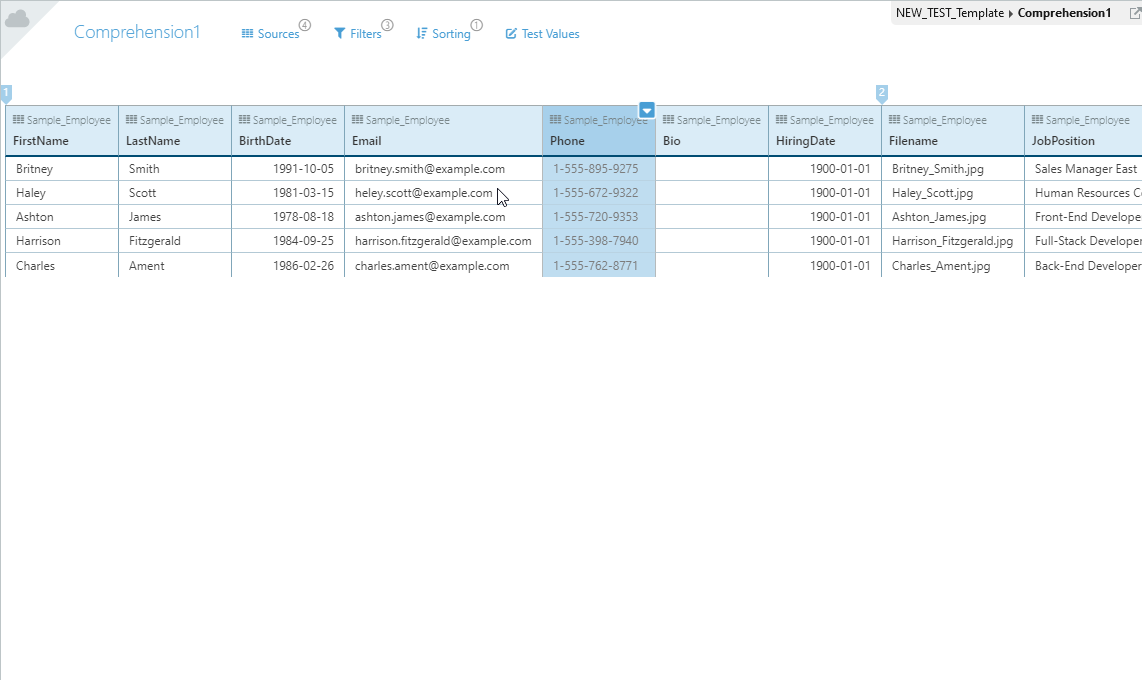
\includegraphics[width=0.5\linewidth]{ss-existing-layout}}%
    \subcaptionbox{Sources Tab\label{fig:ss_existing_layout_sources}}%
      {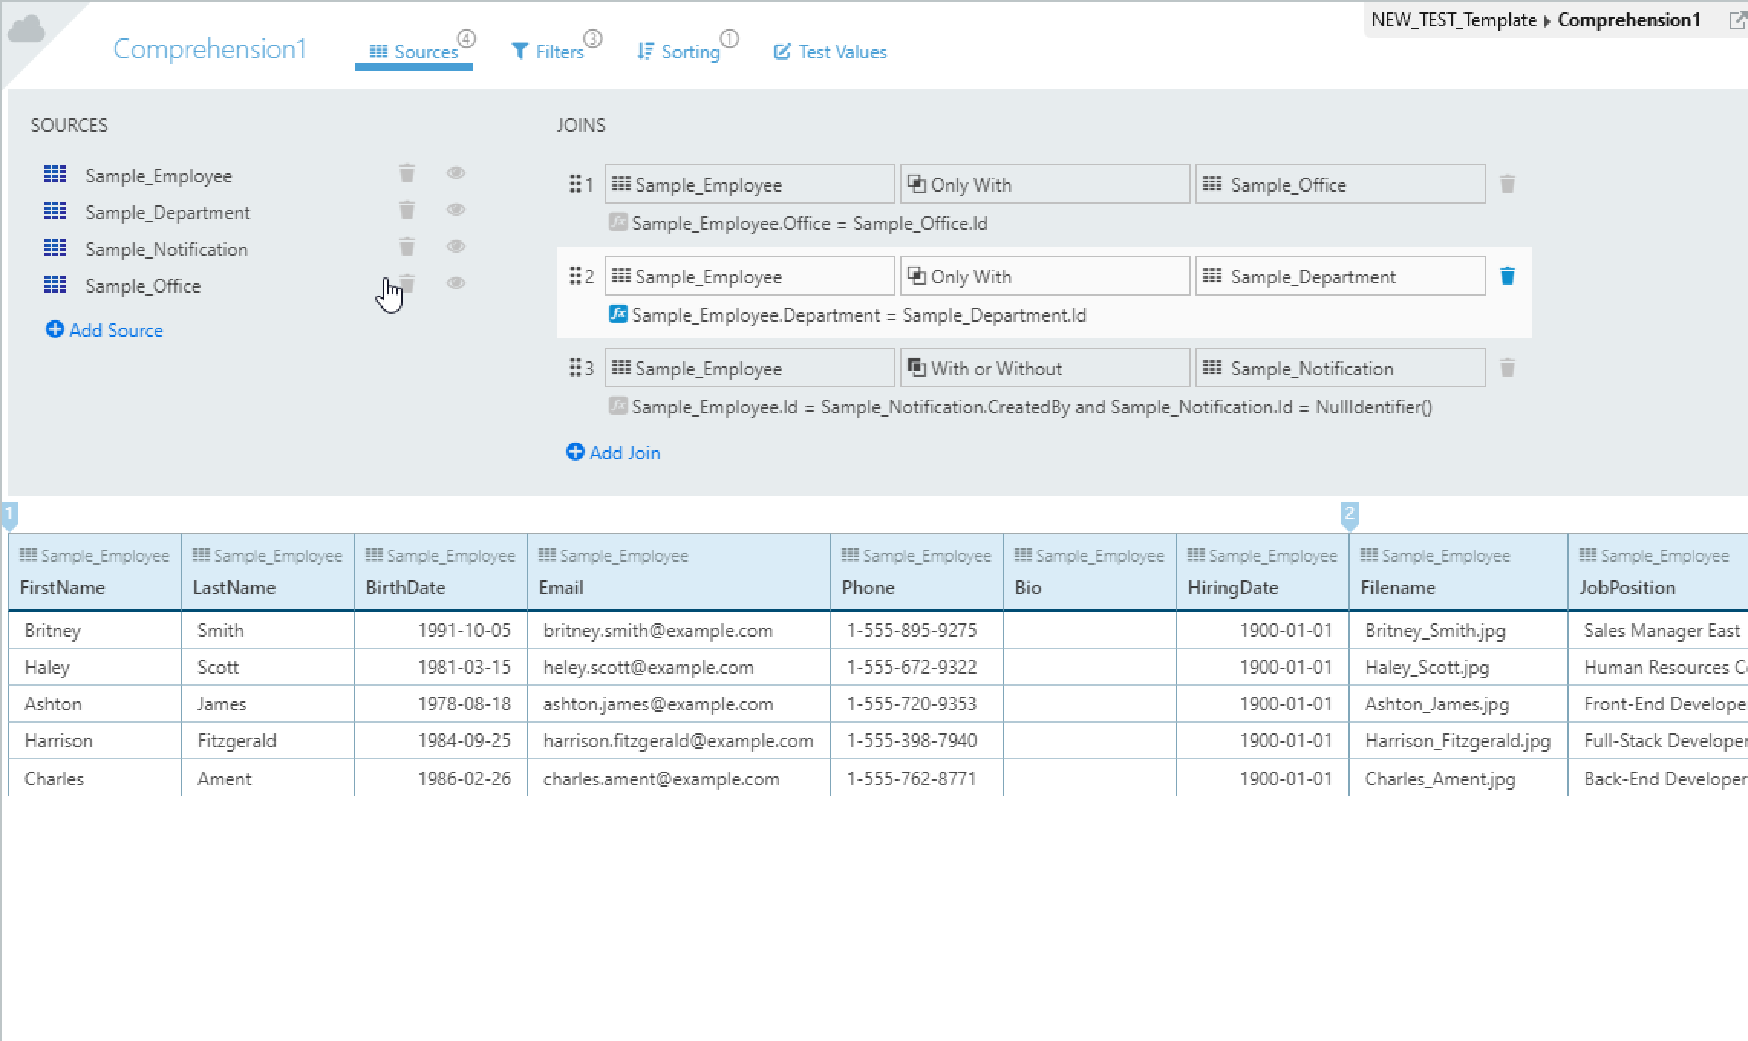
\includegraphics[width=0.5\linewidth]{ss-existing-layout-sources}}%
      \\
    \subcaptionbox{Filters Tab\label{fig:ss_existing_layout_filters}}%
    {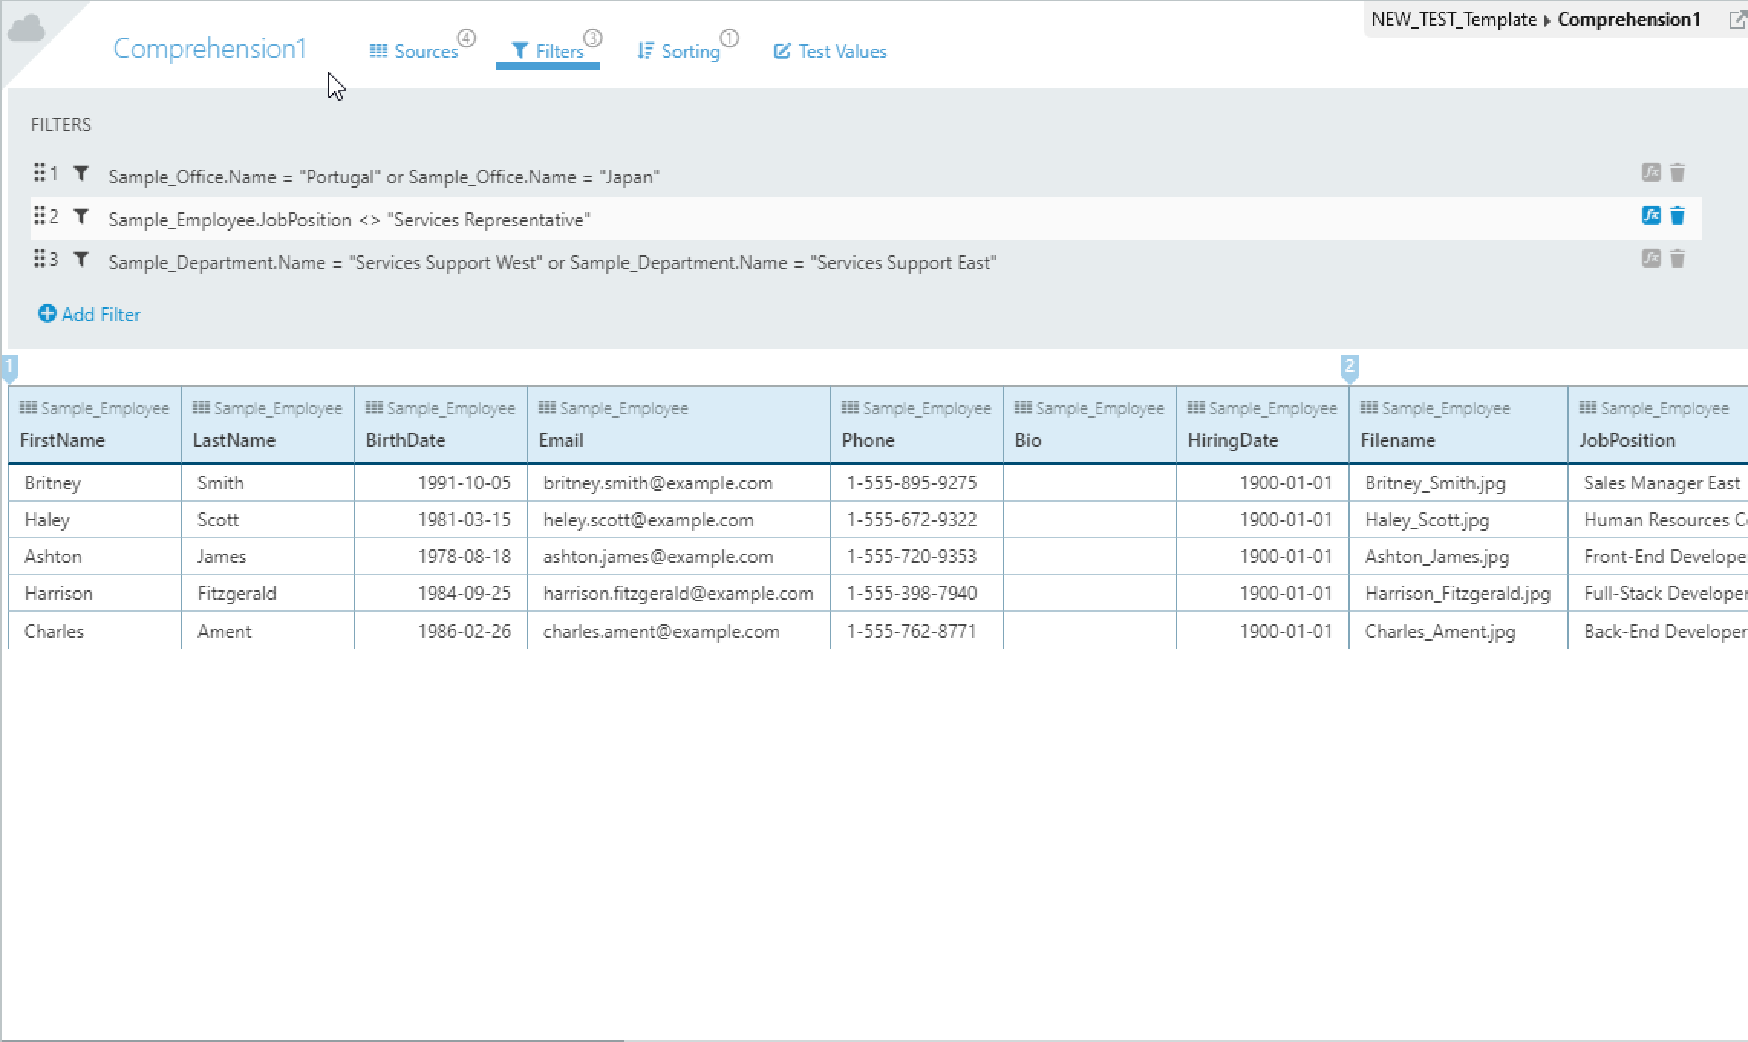
\includegraphics[width=0.5\linewidth]{ss-existing-layout-filters}}%
  \subcaptionbox{Sorting Tab\label{fig:ss_existing_layout_sorting}}%
    {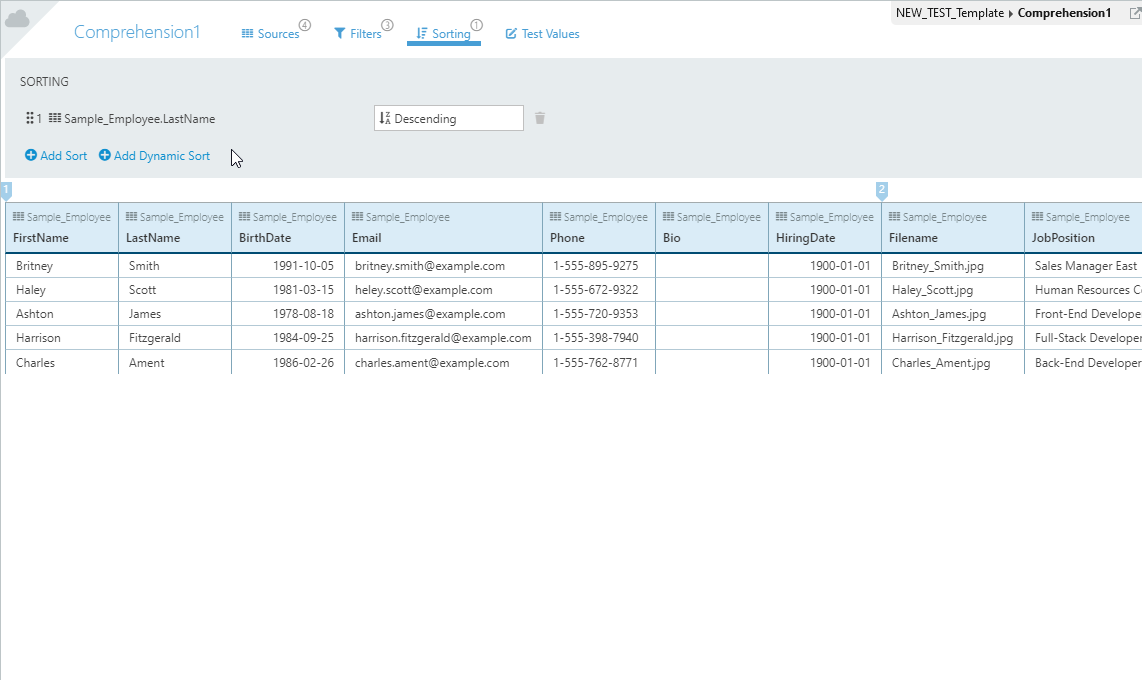
\includegraphics[width=0.5\linewidth]{ss-existing-layout-sorting}}%
  \caption{Example of a database query representation through the existing visual interface.}
    \label{fig:example_of_query_representation}
\end{figure}

Therefore, the designing of a new general layout where it is possible to view the most important query components at once was considered a major requirement. A solid improvement regarding that, could optimize not only the time and effort required to comprehend queries but also to formulate them, since all information is more visible and accessible.

There was also a concern to build a layout that does not compromise the system usability for more complex cases, such as queries that contain a relevant number of entities or conditions.

Accordingly, some wireframes were sketched in order to percept how the query components could be jointly combined in a unique view. Figure \ref{fig:sketch_wireframes} illustrates the two options elected from multiple approaches explored.

In both options, there are two principal areas in the interface as it was before: the query editor area and the preview of the query result. However, it was explored two new manners to display all information of editors jointly with the query result preview. In \nameref{fig:sketch_wireframe_a}, the sub-editors remain in the top area and the query result preview below. The \nameref{fig:sketch_wireframe_b} illustrates another possibility sketched where all editors are presented on the left side of the screen and the visualization of the results are presented on the right side.

\begin{figure}[tb]
  \centering
  \subcaptionbox{Option A\label{fig:sketch_wireframe_a}}%
    {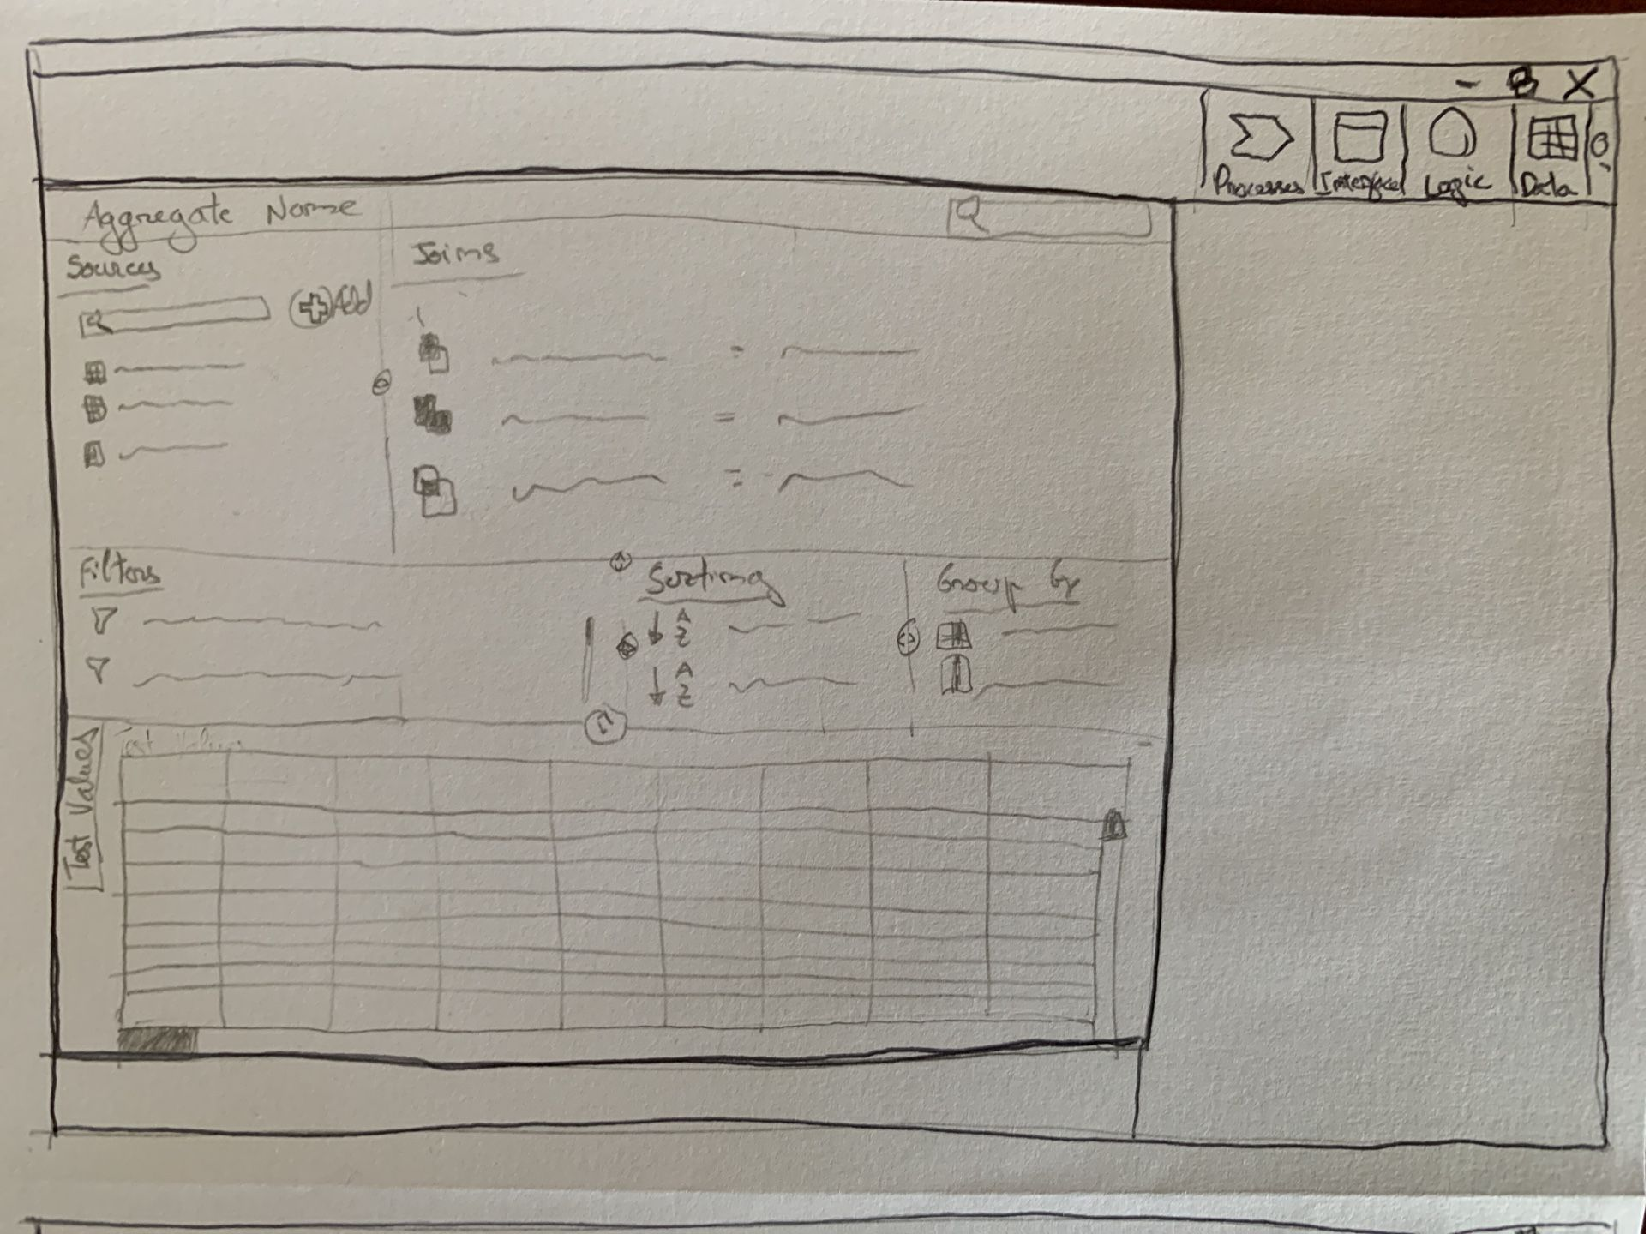
\includegraphics[width=0.5\linewidth]{sketch-wireframe-a}}%
  \subcaptionbox{Option B\label{fig:sketch_wireframe_b}}%
  {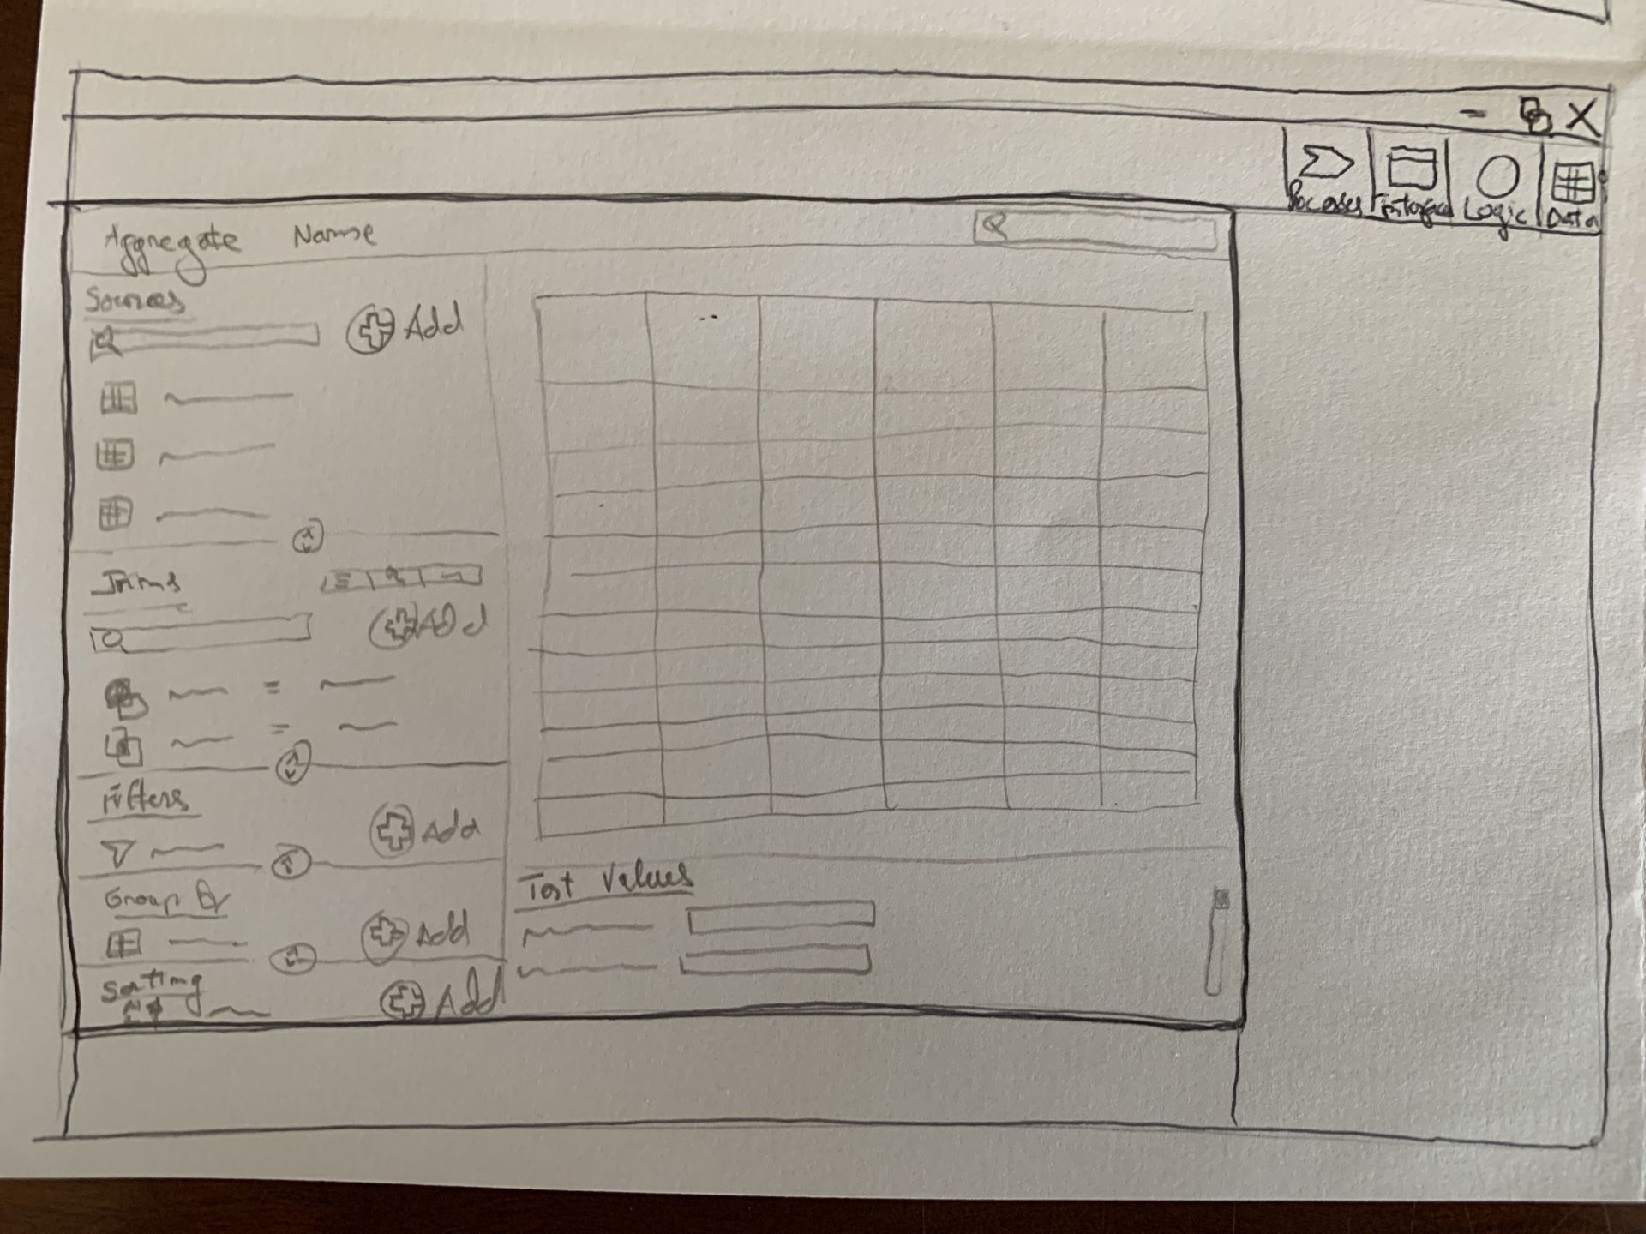
\includegraphics[width=0.5\linewidth]{sketch-wireframe-b}}%
\caption{Interface layout sketches.}
  \label{fig:sketch_wireframes}
\end{figure}

Regardless of the option, the layouts presented have in a single view the most important aspects to understand what query is built.

Beyond the disposition of the different interface views and components, other features were sketched in order to think more about it and structure concrete ideas to implement it.

The existing interface has no mechanism that allows the user to easily find the data of an entity or attribute. The attributes included in the query were not represented in any region of the interface beyond the query result table. Thereby, the unique way to find out the attribute is looking for in each table header, using the horizontal scroll, until the intended attribute is found. That process is cumbersome and slow, so that there was sketched an alternative that includes the attributes in the sources view. Consequently, users can click on attributes and the attribute will be highlighted automatically in the query result preview, as illustrated in Figure \ref{fig:sketchAttributeSearch}. Also, the idea of a search engine was considered, so that users can search for an entity or attribute faster.

\begin{figure}[htbp]
	\centering
	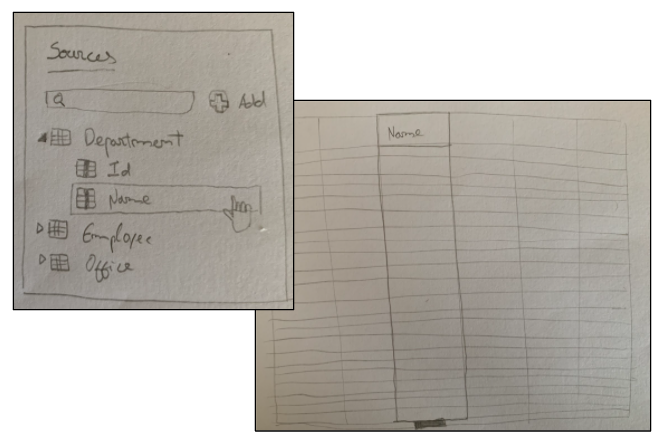
\includegraphics[height=2.5in]{sketch-attribute-search}
	\caption{Searching for an attribute data on the query output preview.}
	\label{fig:sketchAttributeSearch}
\end{figure}

Furthermore, different approaches more compact and functional were explored to display the joins used in the query. Figure \ref{fig:sketch-joins} shows the idea sketched to represent joins in three different lists: a simple list of all join operations inside the query, and two other ones aggregated by the entities involved by the join kind.

\begin{figure}[tb]
  \centering
  \subcaptionbox{Joins flat list\label{fig:sketch-joins-list}}%
    {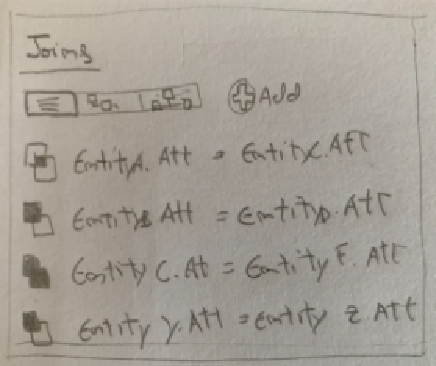
\includegraphics[width=0.3\linewidth]{sketch-joins-list}}%
  \subcaptionbox{Joins associated to each entity\label{fig:sketch-joins-by-entity}}%
  {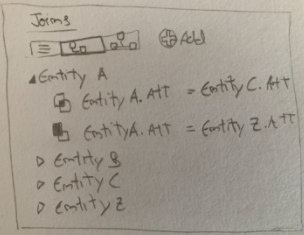
\includegraphics[width=0.3\linewidth]{sketch-joins-by-entity}}%
  \subcaptionbox{Joins by each join kind\label{fig:sketch-joins-by-kind}}%
  {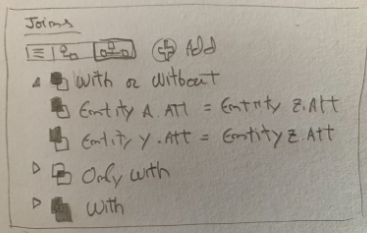
\includegraphics[width=0.3\linewidth]{sketch-joins-by-kind}}%
\caption{Sketches elaborated to explore other approaches to represent the join operations present in the query.}
  \label{fig:sketch_joins}
\end{figure}

Lastly, it was sketched an idea to accelerate the searching process of a specific element inside the query. Therefore, the sketch represented in Figure \ref{fig:sketchGeneralSearch} demonstrates an idea taken into account to find all references of an entity. This general search could allow users to find entities, joins, filters, or other query elements faster.

\begin{figure}[htbp]
	\centering
	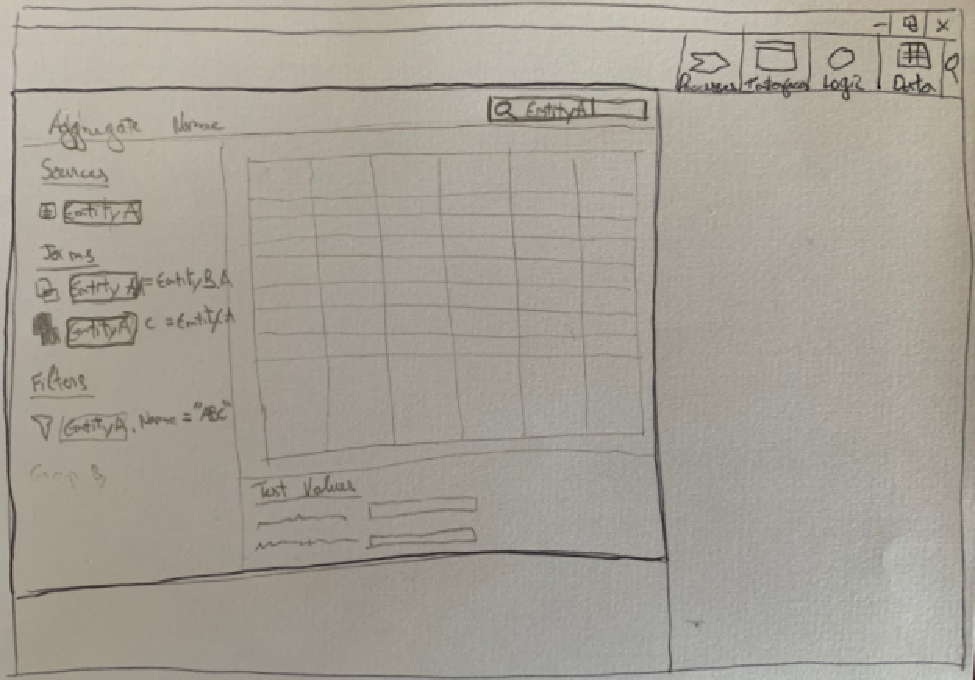
\includegraphics[height=2.5in]{sketch-general-search}
	\caption{Sketch of a general search to allow users to find query elements represented in the interface.}
	\label{fig:sketchGeneralSearch}
\end{figure}

Although the sketched ideas may not be applied to the final result since they depend on the whole iterative design process that started afterward, they were important to move from problem definition to solution design.


\section{Paper Prototype}
\label{sec:paper_prototype}
% Do not forget to refer that due to COVID-19 the Paper Prototype was scanned and mounted as a low-fidelity prototype using InVision App.

\subsection{Design}
\label{subsec:paper_prototype_design}

\subsection{Implementation}
\label{subsec:paper_prototype_implementation}
% It is important to refer the implementation complexity of the prototype in InVision due to the interface complexity.

\subsection{Evaluation}
\label{subsec:paper_prototype_evaluation}
%Comparison with Current Implementation Evaluation


\section{Service Studio Implementation}
\label{sec:service_studio_implementation}

\subsection{Design}
\label{subsec:service_studio_design}

\subsection{Implementation}
\label{subsec:service_studio_implementation}

\subsection{Evaluation}
\label{subsec:service_studio_evaluation}

